\documentclass[tikz]{standalone}

\usetikzlibrary{intersections, decorations.markings}

\tikzset{
    mark rect/.style={
        decoration={markings, mark=at position 0.5 with {
            \draw[draw=black, fill=white] (-6pt,-2pt) rectangle (6pt,2pt);
        }}, postaction={decorate}
    },
    mark one circle/.style={
        decoration={markings, mark=at position 0.5 with {
                \draw[fill=white] (0,0) circle (2pt);
        }}, postaction={decorate}
    },
}

\colorlet{FilledSurface}{blue!20}
\colorlet{FilledSurfaceGroupOne}{blue!20}
\colorlet{FilledSurfaceGroupTwo}{red!20}
\colorlet{FilledSurfaceGroupThree}{green!20}
\colorlet{FilledSurfaceGroupFour}{magenta!20}
\colorlet{FormulaBackground}{green!10}
\colorlet{FormulaFrame}{green}


\begin{document}
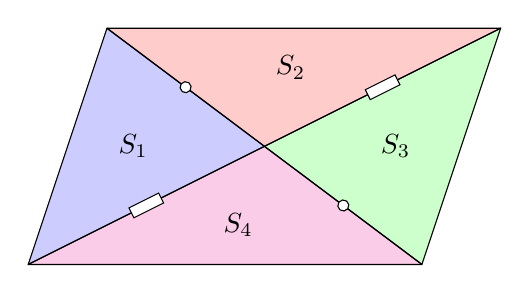
\begin{tikzpicture}

    \coordinate (A) at (0, 0);
    \coordinate (B) at (1, 3);
    \coordinate (C) at (6, 3);
    \coordinate (D) at (5, 0);

    \draw [name path=AC] (A) -- (C);
    \draw [name path=BD] (B) -- (D);
    \path [name intersections={of=AC and BD, by=I}];

    \fill[FilledSurfaceGroupOne] (A) -- (B) -- (I);
    \fill[FilledSurfaceGroupTwo] (B) -- (C) -- (I);
    \fill[FilledSurfaceGroupThree] (C) -- (D) -- (I);
    \fill[FilledSurfaceGroupFour] (A) -- (D) -- (I);

    \node at (barycentric cs:A=1,B=1,I=1) {$S_1$};
    \node at (barycentric cs:B=1,C=1,I=1) {$S_2$};
    \node at (barycentric cs:C=1,D=1,I=1) {$S_3$};
    \node at (barycentric cs:A=1,D=1,I=1) {$S_4$};

    \draw (A) -- (B) -- (C) -- (D) -- cycle;
    \draw (B) -- (D);
    \draw (A) -- (C);


    \draw[mark rect] (A) -- (I);
    \draw[mark rect] (C) -- (I);
    \draw[mark one circle] (B) -- (I);
    \draw[mark one circle] (D) -- (I);


\end{tikzpicture}
\end{document}
